\Chapter{REVUE DE LITTÉRATURE}\label{sec:RevLitt}
% Texte / Text.

\section{Les complexités de développer \texttt{ERP}}
% TODO voir article erp en entreprise
% REF implantation d’un ERP en PME

Le développement d’une solution \texttt{ERP} doit supporter plusieurs niveaux~\cite{uqam_erp_benefice_2008} : 
\begin{enumerate}
    \item Évaluation des besoins;
    \item Préparation du projet;
    \begin{enumerate}
        \item Organisation du projet;
        \item Définir les objectifs;
        \item Créer un plan détaillé;
    \end{enumerate}
    \item Dessin d’affaires;
    \begin{enumerate}
        \item Analyser les processus d’affaires actuels;
        \item Maîtrise du système \texttt{ERP};
        \item Revue des processus;
    \end{enumerate}
    \item Réalisation;
    \begin{enumerate}
        \item Développement technique;
        \item Étude pilote;
    \end{enumerate}
    \item Préparation finale;
    \begin{enumerate}
        \item Réglages et tests;
        \item Éduquer et former la masse critique;
    \end{enumerate}
    \item Mise en production et support;
    \begin{enumerate}
        \item Déploiement des modules \texttt{ERP};
        \item Améliorer et élargir les systèmes \texttt{ERP} de façon continue;
    \end{enumerate}
\end{enumerate}

Autour de ça, il faut mettre en place une gestion du changement et adapter le développement des affaires.

Plusieurs de ces étapes ne sont pas prises au sérieux, tel que le financement. De plus, l’implantation se fait sur une longue période de temps.

Dans Odoo, le nombre de modules augmente avec le temps et diffère entre les versions, une recherche fastidieuse doit être effectué pour réduire le temps de développement à éviter de réinventer la roue.

Il faut adapter les processus des organisations aux fonctionnalités existantes, sinon il est trop coûteux de tout recréer selon les processus de l’entreprise.

En plus de suivre toutes ces étapes, il faut mettre en place une pérennité pour l’amélioration continue sur le projet, ça devient un processus lourd qui doit durer dans le temps.


\section{Logiciel no-code / low-code}

Logiciel no-code / low-code = LCNC

Basé sur des templates de code et un interface qui permet au besoin la configuration par du code.

C’est un concept qui permet à l’utilisateur de développer une plateforme en utilisant pas ou peu de code.

% TODO REF A. C. Bock, U. Frank: Low-Code Platform, Bus Inf Syst Eng 63(6):733–740 (2021)
% TODO REF Supporting the understanding and comparison of low-code development platforms

Besoin de : 
\begin{enumerate}
    \item Aspect général;
    \begin{enumerate}
        \item Gestion des rôles et permissions par des groupes utilisateurs ou individuelle;
        \item Mécanisme de déploiement et exportation;
    \end{enumerate}
    \item Perspective d’intéraction;
    \begin{enumerate}
        \item Mécanisme pour changer le design de l’interface utilisateur;
        \item Mécanisme pour coupler l’interface à un modèle et un contrôleur (\texttt{MVC});
        \item Mécanisme pour faire le rendu visuel sur différents types d’appareils;
    \end{enumerate}
    \item Perspective dynamique;
    \begin{enumerate}
        \item Gestion des processus du système et de la machine;
        \item Composantes de modélisation de processus conceptuel;
        \item Système de gestion des états et des transitions;
    \end{enumerate}
    \item Perspective fonctionnelle;
    \begin{enumerate}
        \item Mécanisme de spécification fonctionnel de base;
        \item Générateur d’algorithme;
        \item Générateur de code de composantes;
        \item Mécanisme d’accès à des API externe;
    \end{enumerate}
    \item Perspective statique;
    \begin{enumerate}
        \item Composante de conception d’un modèle de données;
        \item Composante pour spécifier des structures de données;
        \item Gestion de base de données interne;
        \item Gestion de base de données externes par API;
    \end{enumerate}
\end{enumerate}

Pour supporter une plateforme \texttt{LCNC} :
\begin{enumerate}
    \item Bases de données;
    \item Services externes;
    \item Gestion des modèles de données;
    \item Plateforme collaborative;
    \item Service infonuage (déploiement, audit de performance, gestion des erreurs/traces/événements, gestion des versions);
    \item Générateur de code;
    \item Compilateur et optimiseur de code;
    \item Modeleur d’application;
    \begin{enumerate}
        \item Widget;
        \item Connecteur;
        \item Processus de logique métier;
        \item Capacité de «drag and drop»;
        \item Modèle de données;
        \item Règles de sécurité;
    \end{enumerate}
\end{enumerate}
Critère de qualité d’une plateforme LCNC :
\begin{enumerate}
    \item GUI;
    \item Interoperability support entre services externes et base de données;
    \item Support de la sécurité;
    \item Support d’une plateforme collaborative;
    \item Support sur la réusabilité, pouvoir répété l’utilisation d’une composante dans différents contextes;
    \item Support de la capacité d’un système à maintenir ou à améliorer ses performances;
    \item Mécanisme de spécification de logique du développement des affaires;
    \item Logiciel pour construire des mécanismes;
    \item Support au déploiement;
\end{enumerate}

\section{Génération de code}
TODO

\section{Logiciel Open Source}
Actuellement, une méthode utilisée pour accélérer le développement est le partage de bibliothèque, une fonctionnalité aurait déjà été programmé et le rendre accessible publiquement permet la réduction d’écriture du code pour réaliser une fonctionnalité souhaitée.

L’Open Source permet aussi de supporter l'interopérabilité~\cite{open_interop_2011}, c’est la capacité de différents logiciels d'interagir et communiquer efficacement entre eux sans entraves ni obstacles, il permet à différents systèmes de fonctionner ensemble de manière transparente et harmonieuse même s’ils ont été développés par différentes organisations.

% \section{Logiciel Libre}
% Le logiciel libre entrave l’interopérabilité seulement pour les systèmes non compatibles avec la copyleft. Bien qu’elle prône la liberté du code, elle est restrictive.

% Cette restriction est nécessaire à la protection du développeur et de la communauté. 

% \section{Dev ops}
% Démontrer outil
% TODO image dev ops

% La partie générateur de code répond seulement au besoin création de code du dev ops.

\section{Création d’une communauté}

\subsection{Communication non violente}

Réduire les frictions entre les participants du réseau d’entraide. C’est avec la mise en place d’une méthode de communication non violente~\footnote{\url{https://fr.wikipedia.org/wiki/Communication_non_violente}} formalisée par Marshall B. Rosenberg, voir Figure~\ref{fig:communication_non_violente}.

\begin{figure}[htb]
\centering
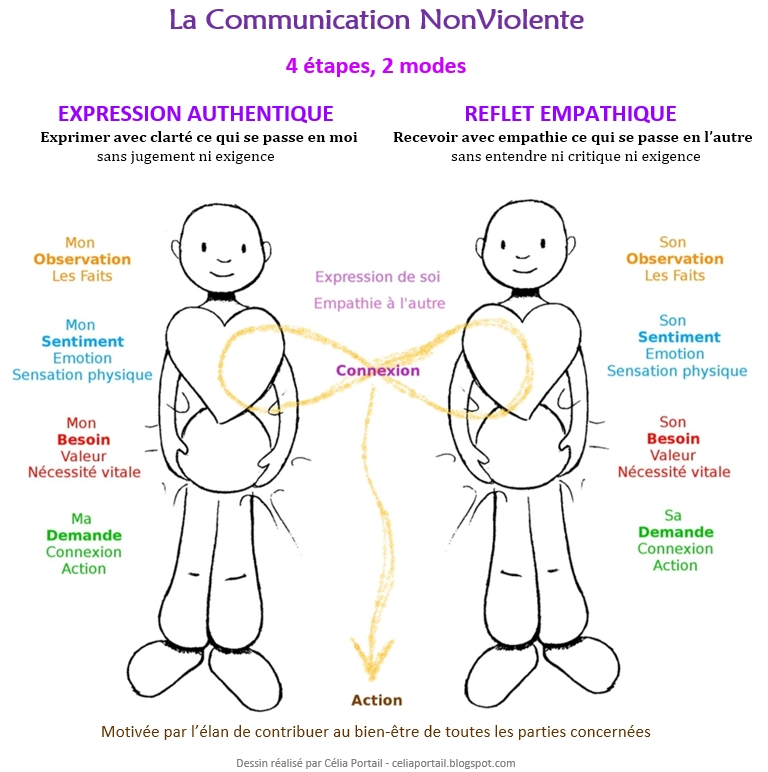
\includegraphics[width=4in]{OSBD_en_CNV.jpg}
\caption{Communication non violente en 4 étapes et 2 modes}
\label{fig:communication_non_violente}
\end{figure}

\subsection{Guide construire une communauté Open Source}
Guide en 4 sections avec des titres indicateurs d’orientation pour un gestionnaire de communauté :

\begin{enumerate}
    \item Mise en place de votre projet pour le succès;
    \item Cultiver votre communauté;
    \item Résoudre les conflits;
    % \item La communauté est le coeur ❤️ de l’open source.
    % \item La communauté est le coeur ❤ de l’open source.
    \item La communauté est le coeur de l’open source.
\end{enumerate}

Il faut :
\begin{enumerate}
    \item rédiger un code de conduite;
    \item proposer la contribution directement sur le projet.
\end{enumerate}
% TODO supporter les autres pages https://opensource.guide/fr/metrics/

Ils n'intègrent ni les aspects de génie industriel qui est vulgarisé avec le guide fusée et ni les critères éthiques de GNU concernant l’hébergement de logiciel.

\subsection{Guide fusée}

Un guide en 7 étapes~\ref{fig:guide_fusee} pour les gestionnaires de projet. Il vous permet de démarrer un projet rapidement qui nécessite une équipe de personnes pour les rendre efficaces dans la réalisation de leurs participations dans le réseau d’entraide.

% REF guide fusée polylabac/cimarlab

\begin{figure}[htb]
\centering
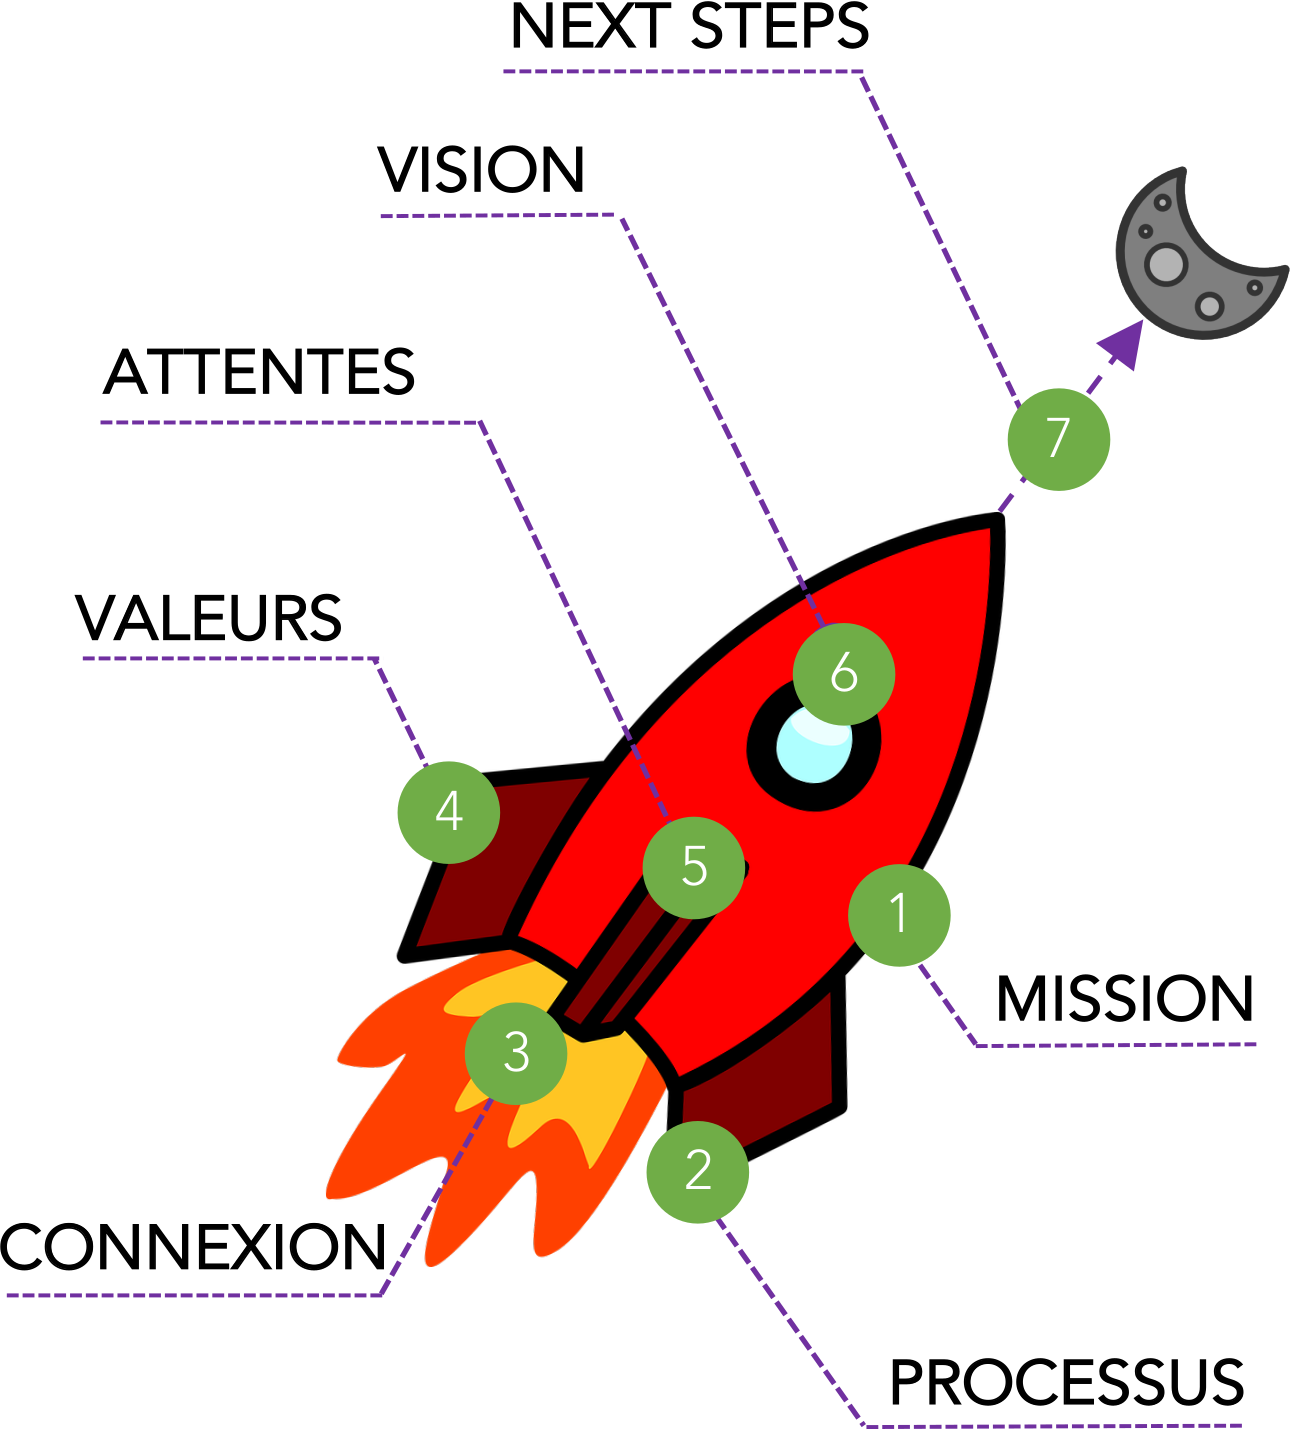
\includegraphics[width=4in]{guide_fusee_definition.png}
\caption{Guide fusée de CimarLab}
\label{fig:guide_fusee}
\end{figure}

\subsection{Critères éthiques de GNU concernant l'hébergement de logiciel}

La licence AGPLv3 n’est pas toujours bien respectée~\cite{violation_libre_2017}.

Les critères éthiques concernant l'hébergement de logiciel~\cite{gnu_critere_hebergement_2022} doivent être accessibles sur les projets de réseau d’entraide. Un guide avec des critères mesurables pour les services destinées à tous ceux qui veulent utiliser un service pour héberger publiquement du code source libre, ainsi qu'éventuellement des programmes exécutables. Ces critères se concentrent sur la protection de la vie privée, le fonctionnement sans JavaScript non libre\footnote{\url{https://www.fsf.org/campaigns/freejs}} , la compatibilité avec les licences à copyleft et leur philosophie, et l'absence de discrimination contre les utilisateurs, quels qu'ils soient.  Les questions à répondre : 

\begin{enumerate}
    \item Est-ce que l'hébergeur fournit l'accès au code source des programmes qu'il héberge?
    \item Est-ce que l'hébergeur permet la redistribution des copies des programmes qu'il héberge?
    \item Est-ce que l'hébergeur permet aux utilisateurs d'apporter des modifications aux programmes qu'il héberge et de les partager avec la communauté?
    \item Est-ce que l'hébergeur impose des restrictions sur l'utilisation ou la redistribution des programmes qu'il héberge?
    \item Est-ce que l'hébergeur respecte les licences de logiciels libres et les droits d'auteur associés aux programmes qu'il héberge?
    \item Est-ce que l'hébergeur fournit des informations sur les licences de logiciels libres et les droits d'auteur associés aux programmes qu'il héberge?
    \item Est-ce que l'hébergeur respecte la vie privée et la sécurité des utilisateurs des programmes qu'il héberge?
    \item Est-ce que l'hébergeur fournit un support et une assistance adéquats aux utilisateurs des programmes qu'il héberge?
\end{enumerate}


% Voir la Figure~\ref{fig:Circuit} pour plus de détails. 

% \begin{figure}[htb]
% \centering
% 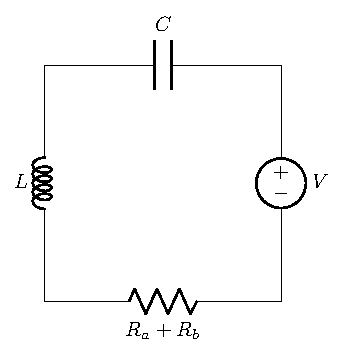
\includegraphics[width=2in]{Circuit_compile}
% \caption{Circuit}
% \label{fig:Circuit}
% \end{figure}